% Options for packages loaded elsewhere
\PassOptionsToPackage{unicode}{hyperref}
\PassOptionsToPackage{hyphens}{url}
%
\documentclass[
]{book}
\usepackage{amsmath,amssymb}
\usepackage{iftex}
\ifPDFTeX
  \usepackage[T1]{fontenc}
  \usepackage[utf8]{inputenc}
  \usepackage{textcomp} % provide euro and other symbols
\else % if luatex or xetex
  \usepackage{unicode-math} % this also loads fontspec
  \defaultfontfeatures{Scale=MatchLowercase}
  \defaultfontfeatures[\rmfamily]{Ligatures=TeX,Scale=1}
\fi
\usepackage{lmodern}
\ifPDFTeX\else
  % xetex/luatex font selection
\fi
% Use upquote if available, for straight quotes in verbatim environments
\IfFileExists{upquote.sty}{\usepackage{upquote}}{}
\IfFileExists{microtype.sty}{% use microtype if available
  \usepackage[]{microtype}
  \UseMicrotypeSet[protrusion]{basicmath} % disable protrusion for tt fonts
}{}
\makeatletter
\@ifundefined{KOMAClassName}{% if non-KOMA class
  \IfFileExists{parskip.sty}{%
    \usepackage{parskip}
  }{% else
    \setlength{\parindent}{0pt}
    \setlength{\parskip}{6pt plus 2pt minus 1pt}}
}{% if KOMA class
  \KOMAoptions{parskip=half}}
\makeatother
\usepackage{xcolor}
\usepackage{color}
\usepackage{fancyvrb}
\newcommand{\VerbBar}{|}
\newcommand{\VERB}{\Verb[commandchars=\\\{\}]}
\DefineVerbatimEnvironment{Highlighting}{Verbatim}{commandchars=\\\{\}}
% Add ',fontsize=\small' for more characters per line
\usepackage{framed}
\definecolor{shadecolor}{RGB}{248,248,248}
\newenvironment{Shaded}{\begin{snugshade}}{\end{snugshade}}
\newcommand{\AlertTok}[1]{\textcolor[rgb]{0.94,0.16,0.16}{#1}}
\newcommand{\AnnotationTok}[1]{\textcolor[rgb]{0.56,0.35,0.01}{\textbf{\textit{#1}}}}
\newcommand{\AttributeTok}[1]{\textcolor[rgb]{0.13,0.29,0.53}{#1}}
\newcommand{\BaseNTok}[1]{\textcolor[rgb]{0.00,0.00,0.81}{#1}}
\newcommand{\BuiltInTok}[1]{#1}
\newcommand{\CharTok}[1]{\textcolor[rgb]{0.31,0.60,0.02}{#1}}
\newcommand{\CommentTok}[1]{\textcolor[rgb]{0.56,0.35,0.01}{\textit{#1}}}
\newcommand{\CommentVarTok}[1]{\textcolor[rgb]{0.56,0.35,0.01}{\textbf{\textit{#1}}}}
\newcommand{\ConstantTok}[1]{\textcolor[rgb]{0.56,0.35,0.01}{#1}}
\newcommand{\ControlFlowTok}[1]{\textcolor[rgb]{0.13,0.29,0.53}{\textbf{#1}}}
\newcommand{\DataTypeTok}[1]{\textcolor[rgb]{0.13,0.29,0.53}{#1}}
\newcommand{\DecValTok}[1]{\textcolor[rgb]{0.00,0.00,0.81}{#1}}
\newcommand{\DocumentationTok}[1]{\textcolor[rgb]{0.56,0.35,0.01}{\textbf{\textit{#1}}}}
\newcommand{\ErrorTok}[1]{\textcolor[rgb]{0.64,0.00,0.00}{\textbf{#1}}}
\newcommand{\ExtensionTok}[1]{#1}
\newcommand{\FloatTok}[1]{\textcolor[rgb]{0.00,0.00,0.81}{#1}}
\newcommand{\FunctionTok}[1]{\textcolor[rgb]{0.13,0.29,0.53}{\textbf{#1}}}
\newcommand{\ImportTok}[1]{#1}
\newcommand{\InformationTok}[1]{\textcolor[rgb]{0.56,0.35,0.01}{\textbf{\textit{#1}}}}
\newcommand{\KeywordTok}[1]{\textcolor[rgb]{0.13,0.29,0.53}{\textbf{#1}}}
\newcommand{\NormalTok}[1]{#1}
\newcommand{\OperatorTok}[1]{\textcolor[rgb]{0.81,0.36,0.00}{\textbf{#1}}}
\newcommand{\OtherTok}[1]{\textcolor[rgb]{0.56,0.35,0.01}{#1}}
\newcommand{\PreprocessorTok}[1]{\textcolor[rgb]{0.56,0.35,0.01}{\textit{#1}}}
\newcommand{\RegionMarkerTok}[1]{#1}
\newcommand{\SpecialCharTok}[1]{\textcolor[rgb]{0.81,0.36,0.00}{\textbf{#1}}}
\newcommand{\SpecialStringTok}[1]{\textcolor[rgb]{0.31,0.60,0.02}{#1}}
\newcommand{\StringTok}[1]{\textcolor[rgb]{0.31,0.60,0.02}{#1}}
\newcommand{\VariableTok}[1]{\textcolor[rgb]{0.00,0.00,0.00}{#1}}
\newcommand{\VerbatimStringTok}[1]{\textcolor[rgb]{0.31,0.60,0.02}{#1}}
\newcommand{\WarningTok}[1]{\textcolor[rgb]{0.56,0.35,0.01}{\textbf{\textit{#1}}}}
\usepackage{longtable,booktabs,array}
\usepackage{calc} % for calculating minipage widths
% Correct order of tables after \paragraph or \subparagraph
\usepackage{etoolbox}
\makeatletter
\patchcmd\longtable{\par}{\if@noskipsec\mbox{}\fi\par}{}{}
\makeatother
% Allow footnotes in longtable head/foot
\IfFileExists{footnotehyper.sty}{\usepackage{footnotehyper}}{\usepackage{footnote}}
\makesavenoteenv{longtable}
\usepackage{graphicx}
\makeatletter
\def\maxwidth{\ifdim\Gin@nat@width>\linewidth\linewidth\else\Gin@nat@width\fi}
\def\maxheight{\ifdim\Gin@nat@height>\textheight\textheight\else\Gin@nat@height\fi}
\makeatother
% Scale images if necessary, so that they will not overflow the page
% margins by default, and it is still possible to overwrite the defaults
% using explicit options in \includegraphics[width, height, ...]{}
\setkeys{Gin}{width=\maxwidth,height=\maxheight,keepaspectratio}
% Set default figure placement to htbp
\makeatletter
\def\fps@figure{htbp}
\makeatother
\setlength{\emergencystretch}{3em} % prevent overfull lines
\providecommand{\tightlist}{%
  \setlength{\itemsep}{0pt}\setlength{\parskip}{0pt}}
\setcounter{secnumdepth}{5}
\usepackage{booktabs}
\ifLuaTeX
  \usepackage{selnolig}  % disable illegal ligatures
\fi
\usepackage[]{natbib}
\bibliographystyle{plainnat}
\IfFileExists{bookmark.sty}{\usepackage{bookmark}}{\usepackage{hyperref}}
\IfFileExists{xurl.sty}{\usepackage{xurl}}{} % add URL line breaks if available
\urlstyle{same}
\hypersetup{
  pdftitle={Genomic Data Analysis Course Exercises},
  pdfauthor={Carson Stacy},
  hidelinks,
  pdfcreator={LaTeX via pandoc}}

\title{Genomic Data Analysis Course Exercises}
\author{Carson Stacy}
\date{2023-10-26}

\usepackage{amsthm}
\newtheorem{theorem}{Theorem}[chapter]
\newtheorem{lemma}{Lemma}[chapter]
\newtheorem{corollary}{Corollary}[chapter]
\newtheorem{proposition}{Proposition}[chapter]
\newtheorem{conjecture}{Conjecture}[chapter]
\theoremstyle{definition}
\newtheorem{definition}{Definition}[chapter]
\theoremstyle{definition}
\newtheorem{example}{Example}[chapter]
\theoremstyle{definition}
\newtheorem{exercise}{Exercise}[chapter]
\theoremstyle{definition}
\newtheorem{hypothesis}{Hypothesis}[chapter]
\theoremstyle{remark}
\newtheorem*{remark}{Remark}
\newtheorem*{solution}{Solution}
\begin{document}
\maketitle

{
\setcounter{tocdepth}{1}
\tableofcontents
}
\hypertarget{about}{%
\chapter{About}\label{about}}

This is a compilation of exercises created for a graduate level course in Genomic Data Analysis at the University of Arkansas.

\hypertarget{usage}{%
\section{Usage}\label{usage}}

Each \textbf{bookdown} chapter is an .Rmd file, and each .Rmd file can contain one (and only one) chapter. A chapter \emph{must} start with a first-level heading: \texttt{\#\ A\ good\ chapter}, and can contain one (and only one) first-level heading.

Use second-level and higher headings within chapters like: \texttt{\#\#\ A\ short\ section} or \texttt{\#\#\#\ An\ even\ shorter\ section}.

The \texttt{index.Rmd} file is required, and is also your first book chapter. It will be the homepage when you render the book.

\hypertarget{render-book}{%
\section{Render book}\label{render-book}}

You can render the HTML version of this example book without changing anything:

\begin{enumerate}
\def\labelenumi{\arabic{enumi}.}
\item
  Find the \textbf{Build} pane in the RStudio IDE, and
\item
  Click on \textbf{Build Book}, then select your output format, or select ``All formats'' if you'd like to use multiple formats from the same book source files.
\end{enumerate}

Or build the book from the R console:

\begin{Shaded}
\begin{Highlighting}[]
\NormalTok{bookdown}\SpecialCharTok{::}\FunctionTok{render\_book}\NormalTok{()}
\end{Highlighting}
\end{Shaded}

To render this example to PDF as a \texttt{bookdown::pdf\_book}, you'll need to install XeLaTeX. You are recommended to install TinyTeX (which includes XeLaTeX): \url{https://yihui.org/tinytex/}.

\hypertarget{preview-book}{%
\section{Preview book}\label{preview-book}}

As you work, you may start a local server to live preview this HTML book. This preview will update as you edit the book when you save individual .Rmd files. You can start the server in a work session by using the RStudio add-in ``Preview book'', or from the R console:

\begin{Shaded}
\begin{Highlighting}[]
\NormalTok{bookdown}\SpecialCharTok{::}\FunctionTok{serve\_book}\NormalTok{()}
\end{Highlighting}
\end{Shaded}

\hypertarget{getting-started-in-r}{%
\chapter{Getting Started in R}\label{getting-started-in-r}}

last updated: 2023-10-26

\hypertarget{installing-packages}{%
\section{Installing Packages}\label{installing-packages}}

First things first: Click the ``Visual'' button in the top-left corner of the code box. This makes the code look more like a word processor. You can always switch back to Source anytime you prefer.

The following code installs a set of R packages used in this document -- if not already installed -- and then loads the packages into R. Note that we utilize the US CRAN repository, but other repositories may be more convenient according to geographic location.

\begin{Shaded}
\begin{Highlighting}[]
\ControlFlowTok{if}\NormalTok{ (}\SpecialCharTok{!}\FunctionTok{require}\NormalTok{(}\StringTok{"pacman"}\NormalTok{)) }\FunctionTok{install.packages}\NormalTok{(}\StringTok{"pacman"}\NormalTok{); }\FunctionTok{library}\NormalTok{(pacman)}

\CommentTok{\# the p\_load function }
\CommentTok{\#    A) installs the package if not installed (like install.packages("package\_name")),}
\CommentTok{\#    B) loads the package (equivalent of library(package\_name))}

\FunctionTok{p\_load}\NormalTok{(}\StringTok{"tidyverse"}\NormalTok{, }\CommentTok{\# An ecosystem of packages for making life in R easier}
       \StringTok{"here"}\NormalTok{, }\CommentTok{\# For locating files easily}
       \StringTok{"knitr"}\NormalTok{, }\CommentTok{\# For generating ("knitting") html or pdf files from .Rmd file}
       \StringTok{"readr"}\NormalTok{, }\CommentTok{\# For faster and easier reading in files to R}
       \StringTok{"pander"}\NormalTok{, }\CommentTok{\# For session info at the end of the document}
       \StringTok{"BiocManager"}\NormalTok{, }\CommentTok{\# For installing Bioconductor R packages}
       \StringTok{"dplyr"} \CommentTok{\# A key part of the tidyverse ecosystem, has useful functions}
\NormalTok{       )}
\end{Highlighting}
\end{Shaded}

\hypertarget{exercise-description}{%
\section{Exercise Description}\label{exercise-description}}

This activity is intended to familiarize you with using RStudio and the R ecosystem to analyze genomic data

\hypertarget{learning-outcomes}{%
\section{Learning outcomes}\label{learning-outcomes}}

At the end of this exercise, you should be able to:

\begin{itemize}
\tightlist
\item
  open, modify, and knit an Rmd file to a pdf/html output
\item
  relate Rmarkdown to a traditional lab notebook
\item
  run commands in an Rmarkdown file
\end{itemize}

\hypertarget{using-r-and-rstudio}{%
\section{Using R and RStudio}\label{using-r-and-rstudio}}

This is an R Markdown document. Markdown is a simple formatting syntax for authoring HTML, PDF, and MS Word documents. For more details on using R Markdown see \url{http://rmarkdown.rstudio.com}.

When you click the \textbf{Knit} button a document will be generated that includes both content as well as the output of any embedded R code chunks within the document. You can embed an R code chunk like this:

\begin{Shaded}
\begin{Highlighting}[]
\CommentTok{\# print a statement}
\FunctionTok{print}\NormalTok{(}\StringTok{"R code in a .Rmd chunk works just like a script"}\NormalTok{)}
\end{Highlighting}
\end{Shaded}

\begin{verbatim}
## [1] "R code in a .Rmd chunk works just like a script"
\end{verbatim}

\begin{Shaded}
\begin{Highlighting}[]
\CommentTok{\# preform basic calculations}
\DecValTok{2}\SpecialCharTok{+}\DecValTok{2}
\end{Highlighting}
\end{Shaded}

\begin{verbatim}
## [1] 4
\end{verbatim}

R is a useful tool for analyzing data. Let's download a data file from GitHub to work with. First, we will download the file manually and open it. Later, we will download the same file directly from the url.

\begin{itemize}
\item
  \href{https://github.com/clstacy/GenomicDataAnalysis_Fa23/blob/main/data/ethanol_stress/msn2-4_mutants_EtOH.txt}{Click here} to open the file in GitHub and click the download icon to download it to your computer.
\item
  Use the ``Import Dataset'' in the Environment panel of RStudio to open the file browser and select the downloaded file

  \begin{itemize}
  \item
    You'll want to use the ``From text (readr)\ldots{}'' option
  \item
    Adjust settings to make sure the file loads in properly.
  \item
    Copy the code that the Import Dataset feature provides for reading in the file and paste it in the code chunk below
  \end{itemize}
\end{itemize}

\begin{Shaded}
\begin{Highlighting}[]
\CommentTok{\# insert here the code used to load the file in from your computer}
\end{Highlighting}
\end{Shaded}

\hypertarget{load-data-directly-from-the-url}{%
\section{Load data directly from the URL}\label{load-data-directly-from-the-url}}

Rather than downloading the file manually and then loading it in from where we downloaded it to, we can just load it directly from the URL, as shown below. A word of caution, this won't work with any URL and you can't guarantee the URL will always work in the future.

\begin{Shaded}
\begin{Highlighting}[]
\CommentTok{\# assign url to a variable}
\NormalTok{DE\_data\_url }\OtherTok{\textless{}{-}} \StringTok{"https://raw.githubusercontent.com/clstacy/GenomicDataAnalysis\_Fa23/main/data/ethanol\_stress/msn2{-}4\_mutants\_EtOH.txt"}

\CommentTok{\# download the data from the web}
\NormalTok{DE\_results\_msn24\_EtOH }\OtherTok{\textless{}{-}}
  \FunctionTok{read\_tsv}\NormalTok{(}\AttributeTok{file=}\NormalTok{DE\_data\_url)}
\end{Highlighting}
\end{Shaded}

\begin{verbatim}
## Warning: One or more parsing issues, call `problems()` on your data frame for details,
## e.g.:
##   dat <- vroom(...)
##   problems(dat)
\end{verbatim}

\begin{verbatim}
## Rows: 5756 Columns: 18
## -- Column specification --------------------------------------------------------
## Delimiter: "\t"
## chr  (3): Gene ID, Common Name, Annotation
## dbl (15): logFC: YPS606 (WT) EtOH response, Pvalue: YPS606 (WT) EtOH respons...
## 
## i Use `spec()` to retrieve the full column specification for this data.
## i Specify the column types or set `show_col_types = FALSE` to quiet this message.
\end{verbatim}

Do remember that this function uses the package readr (a part of the tidyverse package we loaded above). If you don't have that package (1) installed and (2) loaded into your script, it won't work. Thankfully, the p\_load function takes care of both of these simultaneously.

\hypertarget{working-with-data-in-r}{%
\section{Working with data in R}\label{working-with-data-in-r}}

To get a quick summary of our data and how it looks

\begin{Shaded}
\begin{Highlighting}[]
\CommentTok{\# take a quick look at how the data is structured}
\FunctionTok{glimpse}\NormalTok{(DE\_results\_msn24\_EtOH)}
\end{Highlighting}
\end{Shaded}

\begin{verbatim}
## Rows: 5,756
## Columns: 18
## $ `Gene ID`                                <chr> "YMR105C", "YML100W", "YER053~
## $ `Common Name`                            <chr> "PGM2", "TSL1", "PIC2", "NCE1~
## $ Annotation                               <chr> "Phosphoglucomutase", "Large ~
## $ `logFC: YPS606 (WT) EtOH response`       <dbl> 7.5999973, 7.7618280, 6.69400~
## $ `Pvalue: YPS606 (WT) EtOH response`      <dbl> 9.40e-38, 1.04e-35, 3.03e-39,~
## $ `FDR: YPS606 (WT) EtOH response`         <dbl> 3.26e-35, 1.54e-33, 2.07e-36,~
## $ `logFC: YPS606 msn2/4ΔΔ EtOH response`   <dbl> 0.78481798, 0.60949852, 1.735~
## $ `Pvalue: YPS606 msn2/4ΔΔ  EtOH response` <dbl> 3.430000e-06, 8.401730e-04, 4~
## $ `FDR: YPS606 msn2/4ΔΔ  EtOH response`    <dbl> 7.420000e-06, 1.398507e-03, 2~
## $ `logFC: WT v msn2/4ΔΔ: EtOH response`    <dbl> -6.815179, -7.152329, -4.9580~
## $ `Pvalue: WT v msn2/4ΔΔ: EtOH response`   <dbl> 6.34e-32, 2.53e-30, 1.35e-27,~
## $ `FDR: WT v msn2/4ΔΔ: EtOH response`      <dbl> 3.65e-28, 7.28e-27, 2.59e-24,~
## $ `logFC: WT v msn2/4ΔΔ: unstressed`       <dbl> -0.144061475, -0.365016862, -~
## $ `Pvalue: WT v msn2/4ΔΔ: unstressed`      <dbl> 0.350436027, 0.041423492, 0.4~
## $ `FDR: WT v msn2/4ΔΔ:unstressed`          <dbl> 0.998531082, 0.998531082, 0.9~
## $ `logFC: WT v msn2/4ΔΔ: EtOH absolute`    <dbl> -6.959241, -7.517346, -5.0845~
## $ `Pvalue: WT v msn2/4ΔΔ: EtOH absolute`   <dbl> 8.55e-37, 2.04e-35, 3.06e-36,~
## $ `FDR: WT v msn2/4ΔΔ: EtOH absolute`      <dbl> 1.64e-33, 1.96e-32, 3.52e-33,~
\end{verbatim}

We see in the output there are 5756 rows and 18 columns in the data. The same information should be available in the environment panel of RStudio

\hypertarget{seeing-data-in-rstudio}{%
\chapter{Seeing Data in RStudio}\label{seeing-data-in-rstudio}}

If we want to take a closer look at the data, we have a few options. To see just the first few lines we can run the following command:

\begin{Shaded}
\begin{Highlighting}[]
\FunctionTok{head}\NormalTok{(DE\_results\_msn24\_EtOH)}
\end{Highlighting}
\end{Shaded}

\begin{verbatim}
## # A tibble: 6 x 18
##   `Gene ID` `Common Name` Annotation                      logFC: YPS606 (WT) E~1
##   <chr>     <chr>         <chr>                                            <dbl>
## 1 YMR105C   PGM2          Phosphoglucomutase                               7.60 
## 2 YML100W   TSL1          Large subunit of trehalose 6-p~                  7.76 
## 3 YER053C   PIC2          Mitochondrial copper and phosp~                  6.69 
## 4 YPR149W   NCE102        Protein involved in regulation~                  0.714
## 5 YKL035W   UGP1          UDP-glucose pyrophosphorylase ~                  4.42 
## 6 YLR258W   GSY2          Glycogen synthase                                7.52 
## # i abbreviated name: 1: `logFC: YPS606 (WT) EtOH response`
## # i 14 more variables: `Pvalue: YPS606 (WT) EtOH response` <dbl>,
## #   `FDR: YPS606 (WT) EtOH response` <dbl>,
## #   `logFC: YPS606 msn2/4ΔΔ EtOH response` <dbl>,
## #   `Pvalue: YPS606 msn2/4ΔΔ  EtOH response` <dbl>,
## #   `FDR: YPS606 msn2/4ΔΔ  EtOH response` <dbl>,
## #   `logFC: WT v msn2/4ΔΔ: EtOH response` <dbl>, ...
\end{verbatim}

This can be difficult to look at. For looking at data similar to an Excel file, RStudio allows this by clicking on the name of the data.frame in the top right corner of the IDE. We can also view a file by typing \texttt{View(filename)}. To open the data in a new window, click the ``pop out'' button next to ``filter'' just above the opened dataset.

\hypertarget{exploring-the-data}{%
\section{Exploring the data}\label{exploring-the-data}}

This dataset includes the log fold changes of gene expression in an experiment testing the ethanol stress response for the YPS606 strain of \emph{S. cerevisiae} and an \emph{msn2/4ΔΔ} mutant. There are also additional columns of metadata about each gene. In later classes, we will cover the details included, but we can already start answering questions.

\textbf{Using RStudio, answer the following questions:}

\begin{enumerate}
\def\labelenumi{\arabic{enumi}.}
\item
  How many genes are included in this study?
\item
  Which gene has the highest log fold change in the \emph{msn2/4ΔΔ} mutant EtOH response?
\item
  How many HSP genes are differentially expressed (FDR \textless{} 0.01) in unstressed conditions for the mutant?
\item
  Do the genes with the largest magnitude fold changes have the smallest p-values?
\item
  Which isoform of phosphoglucomutase is upregulated in response to ethanol stress? Do you think \emph{msn2/4} is responsible for this difference?
\end{enumerate}

Be sure to knit this file into a pdf or html file once you're finished.

System information for reproducibility:

\begin{Shaded}
\begin{Highlighting}[]
\NormalTok{pander}\SpecialCharTok{::}\FunctionTok{pander}\NormalTok{(}\FunctionTok{sessionInfo}\NormalTok{())}
\end{Highlighting}
\end{Shaded}

\textbf{R version 4.3.1 (2023-06-16)}

\textbf{Platform:} aarch64-apple-darwin20 (64-bit)

\textbf{locale:}
en\_US.UTF-8\textbar\textbar en\_US.UTF-8\textbar\textbar en\_US.UTF-8\textbar\textbar C\textbar\textbar en\_US.UTF-8\textbar\textbar en\_US.UTF-8

\textbf{attached base packages:}
\emph{stats}, \emph{graphics}, \emph{grDevices}, \emph{utils}, \emph{datasets}, \emph{methods} and \emph{base}

\textbf{other attached packages:}
\emph{BiocManager(v.1.30.22)}, \emph{pander(v.0.6.5)}, \emph{knitr(v.1.44)}, \emph{here(v.1.0.1)}, \emph{lubridate(v.1.9.3)}, \emph{forcats(v.1.0.0)}, \emph{stringr(v.1.5.0)}, \emph{dplyr(v.1.1.3)}, \emph{purrr(v.1.0.2)}, \emph{readr(v.2.1.4)}, \emph{tidyr(v.1.3.0)}, \emph{tibble(v.3.2.1)}, \emph{ggplot2(v.3.4.4)}, \emph{tidyverse(v.2.0.0)} and \emph{pacman(v.0.5.1)}

\textbf{loaded via a namespace (and not attached):}
\emph{utf8(v.1.2.3)}, \emph{generics(v.0.1.3)}, \emph{stringi(v.1.7.12)}, \emph{hms(v.1.1.3)}, \emph{digest(v.0.6.33)}, \emph{magrittr(v.2.0.3)}, \emph{evaluate(v.0.22)}, \emph{grid(v.4.3.1)}, \emph{timechange(v.0.2.0)}, \emph{bookdown(v.0.36)}, \emph{fastmap(v.1.1.1)}, \emph{rprojroot(v.2.0.3)}, \emph{fansi(v.1.0.5)}, \emph{scales(v.1.2.1)}, \emph{cli(v.3.6.1)}, \emph{rlang(v.1.1.1)}, \emph{crayon(v.1.5.2)}, \emph{bit64(v.4.0.5)}, \emph{munsell(v.0.5.0)}, \emph{withr(v.2.5.1)}, \emph{yaml(v.2.3.7)}, \emph{parallel(v.4.3.1)}, \emph{tools(v.4.3.1)}, \emph{tzdb(v.0.4.0)}, \emph{colorspace(v.2.1-0)}, \emph{curl(v.5.1.0)}, \emph{vctrs(v.0.6.4)}, \emph{R6(v.2.5.1)}, \emph{lifecycle(v.1.0.3)}, \emph{bit(v.4.0.5)}, \emph{vroom(v.1.6.4)}, \emph{pkgconfig(v.2.0.3)}, \emph{pillar(v.1.9.0)}, \emph{gtable(v.0.3.4)}, \emph{glue(v.1.6.2)}, \emph{Rcpp(v.1.0.11)}, \emph{xfun(v.0.40)}, \emph{tidyselect(v.1.2.0)}, \emph{rstudioapi(v.0.15.0)}, \emph{htmltools(v.0.5.6.1)}, \emph{rmarkdown(v.2.25)} and \emph{compiler(v.4.3.1)}

\hypertarget{cross}{%
\chapter{Cross-references}\label{cross}}

Cross-references make it easier for your readers to find and link to elements in your book.

\hypertarget{chapters-and-sub-chapters}{%
\section{Chapters and sub-chapters}\label{chapters-and-sub-chapters}}

There are two steps to cross-reference any heading:

\begin{enumerate}
\def\labelenumi{\arabic{enumi}.}
\tightlist
\item
  Label the heading: \texttt{\#\ Hello\ world\ \{\#nice-label\}}.

  \begin{itemize}
  \tightlist
  \item
    Leave the label off if you like the automated heading generated based on your heading title: for example, \texttt{\#\ Hello\ world} = \texttt{\#\ Hello\ world\ \{\#hello-world\}}.
  \item
    To label an un-numbered heading, use: \texttt{\#\ Hello\ world\ \{-\#nice-label\}} or \texttt{\{\#\ Hello\ world\ .unnumbered\}}.
  \end{itemize}
\item
  Next, reference the labeled heading anywhere in the text using \texttt{\textbackslash{}@ref(nice-label)}; for example, please see Chapter \ref{cross}.

  \begin{itemize}
  \tightlist
  \item
    If you prefer text as the link instead of a numbered reference use: \protect\hyperlink{cross}{any text you want can go here}.
  \end{itemize}
\end{enumerate}

\hypertarget{captioned-figures-and-tables}{%
\section{Captioned figures and tables}\label{captioned-figures-and-tables}}

Figures and tables \emph{with captions} can also be cross-referenced from elsewhere in your book using \texttt{\textbackslash{}@ref(fig:chunk-label)} and \texttt{\textbackslash{}@ref(tab:chunk-label)}, respectively.

See Figure \ref{fig:nice-fig}.

\begin{Shaded}
\begin{Highlighting}[]
\FunctionTok{par}\NormalTok{(}\AttributeTok{mar =} \FunctionTok{c}\NormalTok{(}\DecValTok{4}\NormalTok{, }\DecValTok{4}\NormalTok{, .}\DecValTok{1}\NormalTok{, .}\DecValTok{1}\NormalTok{))}
\FunctionTok{plot}\NormalTok{(pressure, }\AttributeTok{type =} \StringTok{\textquotesingle{}b\textquotesingle{}}\NormalTok{, }\AttributeTok{pch =} \DecValTok{19}\NormalTok{)}
\end{Highlighting}
\end{Shaded}

\begin{figure}

{\centering 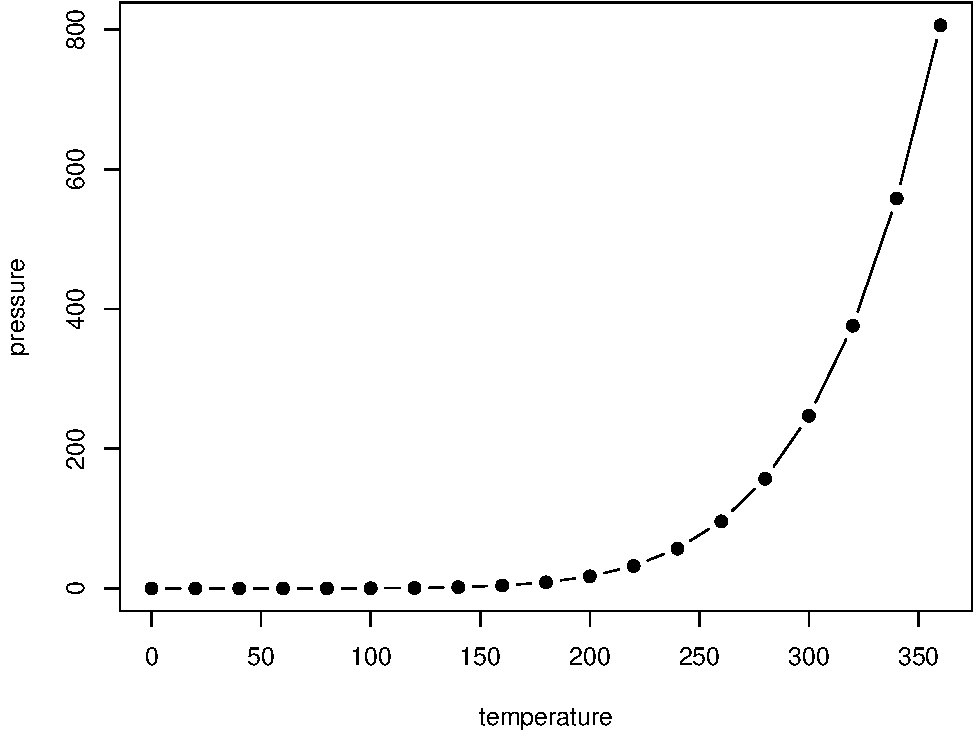
\includegraphics[width=0.8\linewidth]{_main_files/figure-latex/nice-fig-1} 

}

\caption{Here is a nice figure!}\label{fig:nice-fig}
\end{figure}

Don't miss Table \ref{tab:nice-tab}.

\begin{Shaded}
\begin{Highlighting}[]
\NormalTok{knitr}\SpecialCharTok{::}\FunctionTok{kable}\NormalTok{(}
  \FunctionTok{head}\NormalTok{(pressure, }\DecValTok{10}\NormalTok{), }\AttributeTok{caption =} \StringTok{\textquotesingle{}Here is a nice table!\textquotesingle{}}\NormalTok{,}
  \AttributeTok{booktabs =} \ConstantTok{TRUE}
\NormalTok{)}
\end{Highlighting}
\end{Shaded}

\begin{table}

\caption{\label{tab:nice-tab}Here is a nice table!}
\centering
\begin{tabular}[t]{rr}
\toprule
temperature & pressure\\
\midrule
0 & 0.0002\\
20 & 0.0012\\
40 & 0.0060\\
60 & 0.0300\\
80 & 0.0900\\
\addlinespace
100 & 0.2700\\
120 & 0.7500\\
140 & 1.8500\\
160 & 4.2000\\
180 & 8.8000\\
\bottomrule
\end{tabular}
\end{table}

\hypertarget{parts}{%
\chapter{Parts}\label{parts}}

You can add parts to organize one or more book chapters together. Parts can be inserted at the top of an .Rmd file, before the first-level chapter heading in that same file.

Add a numbered part: \texttt{\#\ (PART)\ Act\ one\ \{-\}} (followed by \texttt{\#\ A\ chapter})

Add an unnumbered part: \texttt{\#\ (PART\textbackslash{}*)\ Act\ one\ \{-\}} (followed by \texttt{\#\ A\ chapter})

Add an appendix as a special kind of un-numbered part: \texttt{\#\ (APPENDIX)\ Other\ stuff\ \{-\}} (followed by \texttt{\#\ A\ chapter}). Chapters in an appendix are prepended with letters instead of numbers.

\hypertarget{footnotes-and-citations}{%
\chapter{Footnotes and citations}\label{footnotes-and-citations}}

\hypertarget{footnotes}{%
\section{Footnotes}\label{footnotes}}

Footnotes are put inside the square brackets after a caret \texttt{\^{}{[}{]}}. Like this one \footnote{This is a footnote.}.

\hypertarget{citations}{%
\section{Citations}\label{citations}}

Reference items in your bibliography file(s) using \texttt{@key}.

For example, we are using the \textbf{bookdown} package \citep{R-bookdown} (check out the last code chunk in index.Rmd to see how this citation key was added) in this sample book, which was built on top of R Markdown and \textbf{knitr} \citep{xie2015} (this citation was added manually in an external file book.bib).
Note that the \texttt{.bib} files need to be listed in the index.Rmd with the YAML \texttt{bibliography} key.

The RStudio Visual Markdown Editor can also make it easier to insert citations: \url{https://rstudio.github.io/visual-markdown-editing/\#/citations}

\hypertarget{blocks}{%
\chapter{Blocks}\label{blocks}}

\hypertarget{equations}{%
\section{Equations}\label{equations}}

Here is an equation.

\begin{equation} 
  f\left(k\right) = \binom{n}{k} p^k\left(1-p\right)^{n-k}
  \label{eq:binom}
\end{equation}

You may refer to using \texttt{\textbackslash{}@ref(eq:binom)}, like see Equation \eqref{eq:binom}.

\hypertarget{theorems-and-proofs}{%
\section{Theorems and proofs}\label{theorems-and-proofs}}

Labeled theorems can be referenced in text using \texttt{\textbackslash{}@ref(thm:tri)}, for example, check out this smart theorem \ref{thm:tri}.

\begin{theorem}
\protect\hypertarget{thm:tri}{}\label{thm:tri}For a right triangle, if \(c\) denotes the \emph{length} of the hypotenuse
and \(a\) and \(b\) denote the lengths of the \textbf{other} two sides, we have
\[a^2 + b^2 = c^2\]
\end{theorem}

Read more here \url{https://bookdown.org/yihui/bookdown/markdown-extensions-by-bookdown.html}.

\hypertarget{callout-blocks}{%
\section{Callout blocks}\label{callout-blocks}}

The R Markdown Cookbook provides more help on how to use custom blocks to design your own callouts: \url{https://bookdown.org/yihui/rmarkdown-cookbook/custom-blocks.html}

\hypertarget{sharing-your-book}{%
\chapter{Sharing your book}\label{sharing-your-book}}

\hypertarget{publishing}{%
\section{Publishing}\label{publishing}}

HTML books can be published online, see: \url{https://bookdown.org/yihui/bookdown/publishing.html}

\hypertarget{pages}{%
\section{404 pages}\label{pages}}

By default, users will be directed to a 404 page if they try to access a webpage that cannot be found. If you'd like to customize your 404 page instead of using the default, you may add either a \texttt{\_404.Rmd} or \texttt{\_404.md} file to your project root and use code and/or Markdown syntax.

\hypertarget{metadata-for-sharing}{%
\section{Metadata for sharing}\label{metadata-for-sharing}}

Bookdown HTML books will provide HTML metadata for social sharing on platforms like Twitter, Facebook, and LinkedIn, using information you provide in the \texttt{index.Rmd} YAML. To setup, set the \texttt{url} for your book and the path to your \texttt{cover-image} file. Your book's \texttt{title} and \texttt{description} are also used.

This \texttt{gitbook} uses the same social sharing data across all chapters in your book- all links shared will look the same.

Specify your book's source repository on GitHub using the \texttt{edit} key under the configuration options in the \texttt{\_output.yml} file, which allows users to suggest an edit by linking to a chapter's source file.

Read more about the features of this output format here:

\url{https://pkgs.rstudio.com/bookdown/reference/gitbook.html}

Or use:

\begin{Shaded}
\begin{Highlighting}[]
\NormalTok{?bookdown}\SpecialCharTok{::}\NormalTok{gitbook}
\end{Highlighting}
\end{Shaded}

\hypertarget{hello-bookdown}{%
\chapter{Hello bookdown}\label{hello-bookdown}}

All chapters start with a first-level heading followed by your chapter title, like the line above. There should be only one first-level heading (\texttt{\#}) per .Rmd file.

\hypertarget{a-section}{%
\section{A section}\label{a-section}}

All chapter sections start with a second-level (\texttt{\#\#}) or higher heading followed by your section title, like the sections above and below here. You can have as many as you want within a chapter.

\hypertarget{an-unnumbered-section}{%
\subsection*{An unnumbered section}\label{an-unnumbered-section}}
\addcontentsline{toc}{subsection}{An unnumbered section}

Chapters and sections are numbered by default. To un-number a heading, add a \texttt{\{.unnumbered\}} or the shorter \texttt{\{-\}} at the end of the heading, like in this section.

  \bibliography{book.bib,packages.bib}

\end{document}
